\section{Tema 3: Conservación de la masa}
\subsection{Teorema del transporte de Reynolds}
\begin{figure}[H]
	\centering
	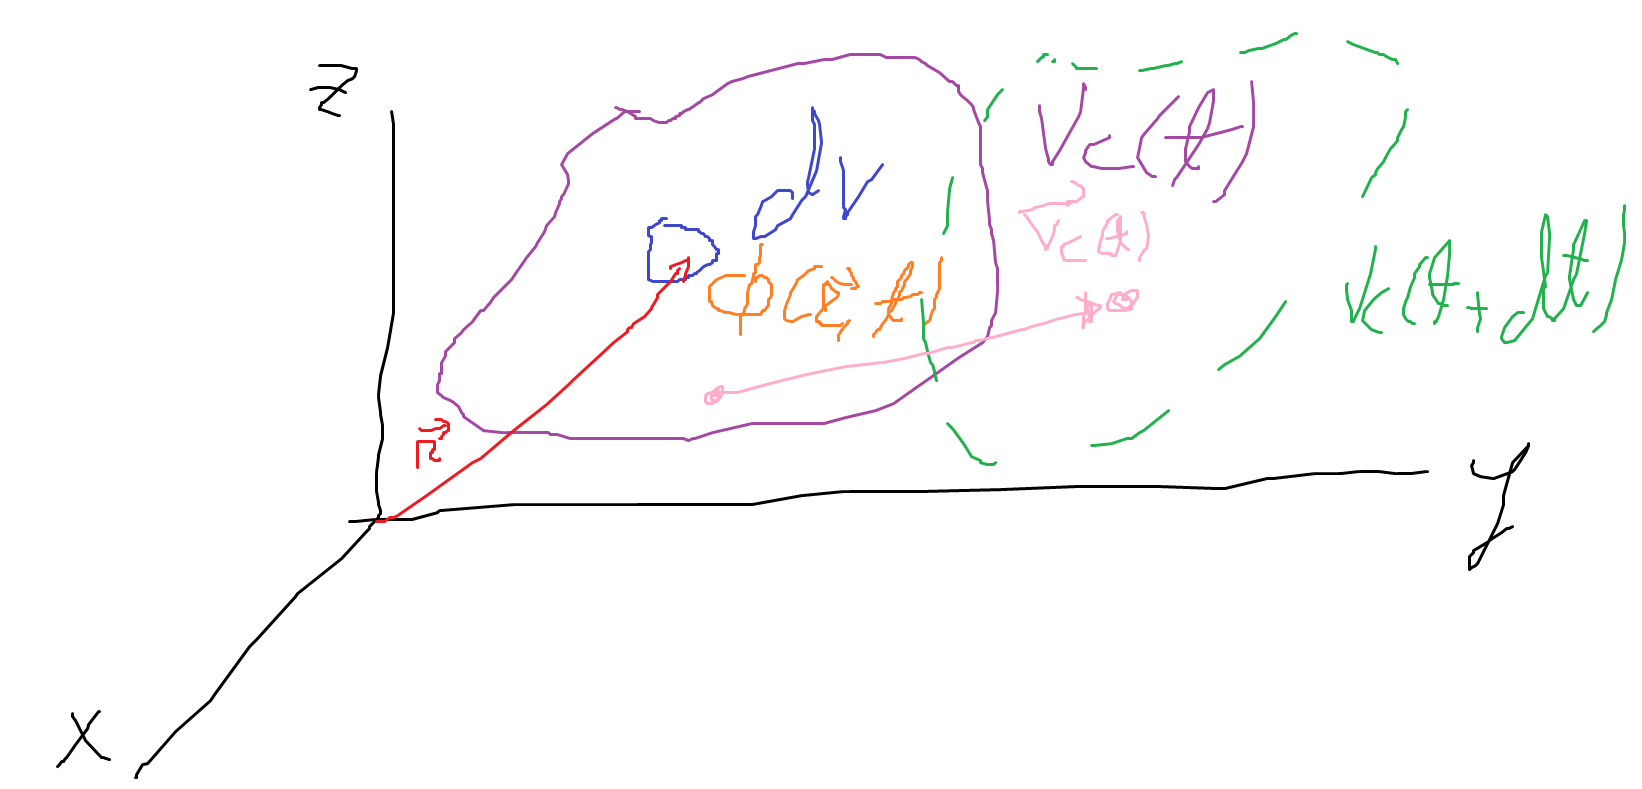
\includegraphics[width=0.7\linewidth]{imagenesTema3/magnitudesReynolds}
	\caption{}
	\label{fig:magnitudesreynolds}
\end{figure}

\[\Phi=\text{Función que depende del espacio y tiempo en general}\rightarrow\Phi=f(\vec{r},t)\]

Nos interesa conocer:
\[\frac{d}{dt}\int_{V_c(t)} \Phi(\vec{r},t) \,dV=\lim_{\Delta t \to 0} \left[\int_{V_c(t+dt)} \Phi(\vec{r},t+dt) \,dV-\int_{V_c(t)} \Phi(\vec{r},t) \,dV\right]\]
Se hace el desarrollo de Taylor en t del primer término:
\[\frac{d}{dt}\int_{V_c(t)} \Phi(\vec{r},t) \,dV=\int_{V_c(t)} \frac{\partial}{\partial t}\Phi(\vec{r},t) \,dV+\lim_{\Delta t \to 0} \frac{1}{\Delta t}\left[\int_{V_c(t+dt)} \Phi(\vec{r},t) \,dV-\int_{V_c(t)} \Phi(\vec{r},t) \,dV\right]\]

Hay que estudiar la velocidad del volumen de control de tal manera que, solo afecta la velocidad paralela a la normal porque es lo que provoca expansión o compresión del mismo, la velocidad tangencial lo "gira":
\[dV=\vec{v}_c\cdot\vec{n}dS\Delta t\]
Por tanto:
\[\frac{d}{dt}\int_{V_c(t)} \Phi(\vec{r},t) \,dV=\int_{V_c(t)} \frac{\partial}{\partial t}\Phi(\vec{r},t) \,dV+\oint_{S_c(t)} \Phi(\vec{r},t)\vec{v}_c\cdot\vec{n}\Delta t \,dS\]

Si queremos podemos imponer que (hablando en tema de volumen fluido):
\[V_c(t)=V_{fluido}(t)=V_f(t)\]
\[\frac{d}{dt}\int_{V_f(t)} \Phi(\vec{r},t) \,dV=\int_{V_f(t)} \frac{\partial}{\partial t}\Phi(\vec{r},t) \,dV+\oint_{S_f(t)} \Phi(\vec{r},t)\vec{v}\cdot\vec{n}\Delta t \,dS\]

Si tomamos un tiempo t* paramétrico tal que $V_c(t*)=V_F(t*) \rightarrow \int_{V_c(t*)}\frac{\partial \Phi}{\partial t}\,dV\approx \int_{V_f(t*)}\frac{\partial \Phi}{\partial t}\,dV$ Solo en ese instante t*

Si se restan las ecuaciones de Volumen de control y la de los movimientos fluidos queda (Teorema de Reynolds del transporte (problemas)):

\[\frac{d}{dt}\int_{V_f(t)}\Phi(\vec{r},t)\,dV=\frac{d}{dt}\int_{V_c(t)}\Phi(\vec{r},t)\,dV+\oint_{S_c(t)} \Phi(\vec{r},t)\left[(\vec{v}-\vec{v}_c)\cdot\vec{n}\right]\Delta t \,dS\]

(TH Reynolds para teoria)
\[\frac{d}{dt}\int_{V_f(t)} \Phi(\vec{r},t) \,dV=\int_{V_f(t)} \frac{\partial}{\partial t}\Phi(\vec{r},t) \,dV+\oint_{S_f(t)} \Phi(\vec{r},t)\vec{v}\cdot\vec{n}\Delta t \,dS\]

Término de variación local:
\[\int_{V_f(t)} \frac{\partial}{\partial t}\Phi(\vec{r},t) \,dV\]
Térimno de variación convectiva:
\[\oint_{S_f(t)} \Phi(\vec{r},t)\vec{v}\cdot\vec{n}\Delta t \,dS\]


Si la magnitud $\Phi = \rho$ Se obtiene la ecuación de conservación de la masa en forma integral:
Es igual a 0 porque no se pierde masa:
(Problemas)
\[\frac{d}{dt}\int_{V_f(t)}\rho\,dV=\frac{d}{dt}\int_{V_c(t)}\rho\,dV+\oint_{S_c(t)} \rho\left[(\vec{v}-\vec{v}_c)\cdot\vec{n}\right]\Delta t \,dS=0\]
(Teoría)
\[\frac{d}{dt}\int_{V_f(t)} \rho \,dV=\int_{V_f(t)} \frac{\partial \rho}{\partial t} \,dV+\oint_{S_f(t)} \rho\vec{v}\cdot\vec{n}\Delta t \,dS=0\]

Si $V_f(t)\approx dV_f(t)$ entonces y aplicando el teorema de gauss se llega a la ecuación diferencial de la masa o forma conservativa:
($\oint_S \varphi \cdot \vec{n}\,dS=\int_V \vec{\nabla}\cdot\varphi\,dV$)
\[\lim_{dV \to 0}\left[\frac{\partial \rho}{\partial t} dV+\vec{\nabla}\cdot\left(\rho\vec{v}\right)dV\right]=0\]
\[\frac{\partial \rho}{\partial t} +\vec{\nabla}\cdot\left(\rho\vec{v}\right)=0\]
Término local de masa: 
\[\frac{\partial \rho}{\partial t}\]
Término convectivo de masa:
\[\vec{\nabla}\cdot\left(\rho\vec{v}\right)\]
